\subsection{Autentica\c{c}\~ao de conte\'udo}
\label{subsection:autenticacao_conteudo}
Dentro de autentica\c{c}\~ao de conte\'udo h\'a uma gama de valida\c{c}\~oes que s\~ao ou que podem ser utilizadas, \cite{wein2012content} e \cite{leighton2007html} s\~ao duas delas.
\paragraph{}
Aqui iremos focar em uma chamada \textit{control DRM-encoded}, que \'e o m\'etodo mais utilizado hoje em dia. Utilizado inclusive por sistemas como Netfilx e VOD de operadoras de TV.
\paragraph{}
Esse processo est\'a intrinsecamente ligado ao processo de autentica\c{c}\~ao de usu\'ario explicado anteriormente. Nele o conte\'udo passa por uma s\'erie de valida\c{c}\~oes antes de tocar.
\paragraph{}
A primeira etapa do processo para tocar o conte\'udo \'e a etapa de \textbf{\textit{License Acquisition}}. Nela, apresentado por \cite{pomelo2009analysis}, antes de tocar \'e feito:
\begin{itemize}
\item Passo 1 -  A aplica\c{c}\~ao requisita do servidor um peda\c{c}o do conte\'udo. Este o retorna com o conte\'udo criptografado.
\item Passo 2 - O cliente l\^e o cabe\c{c}alho do conte\'udo criptografado e determina que aquele conte\'udo \'e criptografado. Para descriptografar o conte\'udo \'e necess\'ario que este tenha recebido a chave do servidor de licen\c{c}a. Caso n\~ao tenha recebido ele envia uma requisi\c{c}\~ao para adquiri-la. Se for a primeira vez que \'e feita a valida\c{c}\~ao da chave ele passa por um processo de \textit{individualization}. Que ser\'a explicado logo mais a frente.(figura \ref{figura:individualization}).
\item Passo 3 - O cliente recebe a licen\c{c}a do servidor, que antes de enviar a chave faz todo o processo de autencidade necess\'ario.
\item Passo 4 - O cliente ap\'os receber a chave pode tocar o conte\'udo. Isso se ele estiver licen\c{c}a para tal, \'e claro.
\end{itemize}

No passo 1 fica claro entender quando em \ref{subsec:vod} explicamos como \'e composto um VOD e qual o seu fluxo de comportamento.
\paragraph{}
No passo 2 o servidor de licen\c{c}a \'e o servidor que faz parte do rol de servidores citados em \ref{subsection:definicoes_seguranca}. O disparo do fluxo do \textit{individualization} \'e feito pela pr\'opia aplica\c{c}\~ao do cliente, que verifica caso o cliente n\~ao possua nenhuma licen\c{c}a ele aponta para um terceiro servidor, onde esse vai retornar com uma licen\c{c}a individual que ser\'a utilizada na hora de validar e tocar conte\'udo. O fluxo do processo \'e apresentado na figura \ref{figura:individualization}. 
\paragraph{}
Todo esse processo de troca de informa\c{c}\~oes \'e feito utilizando trocas de chaves assim\'etricas p\'ublicas garantindo assim a seguran\c{c}a e proced\^encia da informa\c{c}\~ao.
\begin{figure}[H]
\caption{autenticacao conte\'udo - \textit{individualization}}
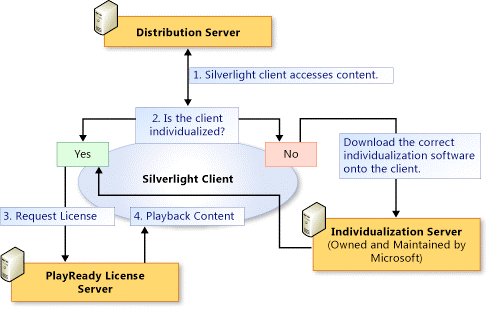
\includegraphics[height=9cm]{Figuras/autenticacao_conteudo_individualization.png} 
\label{figura:individualization}
\end{figure}
Ap\'os \textbf{\textit{License Acquisition}} o \textit{player} est\'a apto a tocar o conte\'udo. A comunica\c{c}\~ao agora \'e feita somente com o servidor de conte\'udo. Recebendo o conte\'udo criptografado e tocando atrav\'es do processo de \textbf{\textit{License Acquisition}}.